%\UseRawInputEncoding
\documentclass{article}
\setcounter{secnumdepth}{0}
\usepackage[T1]{fontenc}
\usepackage[utf8]{inputenc}
%\usepackage[latin1]{inputenc}
%\usepackage[english, norsk]{babel}
\usepackage{filecontents}
\usepackage{tcolorbox}
\usepackage{url}
\usepackage{etoolbox}
\usepackage{framed}
\usepackage{framed, color}
\usepackage{xcolor}
\usepackage{mdframed}
\usepackage{float}
\usepackage{gensymb}
\usepackage{amsmath}
\usepackage{amsfonts}

\definecolor{Black}{rgb}{0.0, 0.0, 0.0}

%Definer kode
\usepackage{listings}
\usepackage{color}
\definecolor{dkgreen}{rgb}{0,0.6,0}
\definecolor{gray}{rgb}{0.5,0.5,0.5}
\definecolor{mauve}{rgb}{0.58,0,0.82}

\lstset{frame=tb,
extendedchars = true,
texcl=true,
  language=C++,
  aboveskip=3mm,
  belowskip=3mm,
  showstringspaces=false,
  columns=flexible,
  basicstyle={\small\ttfamily},
  numbers=none,
  numberstyle=\tiny\color{gray},
  keywordstyle=\color{blue},
  commentstyle=\color{dkgreen},
  stringstyle=\color{mauve},
  breaklines=true,
  breakatwhitespace=true,
  tabsize=3
}

\usepackage[colorlinks]{hyperref}
\hypersetup{citecolor=Black}
\hypersetup{linkcolor=Black}
\hypersetup{urlcolor=Black}
\usepackage{cleveref}


\setlength{\parindent}{0em}
\setlength{\parskip}{1em}
%\renewcommand{\baselinestretch}{2.0}

%\renewcommand\thesubsection{\alph{subsection}}

\renewcommand{\figurename}{Figure}
\begin{document}
\author{Kent Odde}
\title{Home Exam\\RFMA310}

\maketitle
\thispagestyle{empty}
\begin{center}
\includegraphics[width=\linewidth,height=0.2\textheight,keepaspectratio]{img/USN.png}
\end{center}
\newpage

\tableofcontents

\newpage

\section{Abstract}
This is my submission for the home exam in Discrete Mathmatics, fall 2020.

%Innholdsfortegnelse
\section{Introduction}
The assignment consists of implementing the ElGamal encryption algorithm, in a programming language of my own choosing. As a requirement for the implementation is speed, I found the most suitable language for the task to be C++. As it happens, this is also the language I'm most proficient in.

One downsize of using C++ is the fact that there exists no built in support for large numbers. Building my own library for this would be too time-consuming, so I decided to make use of the Gnu Multiple Precision library (GMP)\cite{GMP}.

Quite a bit of overhead were required to encrypt larger inputs. However, because this course is concerned with the mathematics behind ElGamal and the fact that the professor wanted a short paper, I will not cover this part of the implementation to a detailed extent.

\subsection{ElGamal}
ElGamal is an asymmetric encryption scheme based on Diffie-Hellman. Asymmetric means that the algorithm uses two different keys for encryption and decryption. As encouraged by the professor, I have used the Wikipedia article\cite{WIKI} as my main source of information on ElGamal. Instead of reiterating the details of the algorithm from the article, I will just focus on the main points here.

We choose a cyclic group G, with a generator g. The private key is denoted by \textit{x}. We use the private key to generate an element of the public key, \textit{h}:

\begin{equation*}
h := g^{x}
\end{equation*}

If we choose a bad g, the discrete logarithm problem, which gives ElGamal its security, will decrease in complexity, resulting in a much less secure implementation.

Choosing a good g, is a field of its own, and beyond the scope of this assigment. The main point is that the g we choose, needs to be able to generate all the elements of the group G.

To illustrate this, lets have a look at the group

\begin{equation*}
  G =((\mathbb{Z}/7)^{*}, \cdot)
\end{equation*}


If we set up a table, where the rows list x values, and the colums list g values, and look at what happens for

\begin{equation*}
  g^{x} \bmod 7
\end{equation*}
it will look like this:

\begin{center}
 \begin{tabular}{||c|c c c c c c||}
 \hline
   x \textbackslash g & 1 & 2 & \textbf{3} & 4 & \textbf{5} & 6\\ [0.5ex]
 \hline
   1 & 1 & 2 & 3 & 4 & 5 & 6 \\
 \hline
   2 & 1 & 4 & 2 & 2 & 4 & 1 \\
 \hline
   3 & 1 & 1 & 6 & 1 & 6 & 6 \\
 \hline
   4 & 1 & 2 & 4 & 4 & 2 & 1 \\
 \hline
   5 & 1 & 4 & 5 & 2 & 3 & 6 \\
 \hline
   6 & 1 & 1 & 1 & 1 & 1 & 1 \\ [1ex]
 \hline
\end{tabular}
\end{center}

As we can see, the only two values for g that generate cyclic groups, are 3 and 5. The rest of them are repeating within a subset.

In our implementation we will pick a static g (and a static p for that matter), from online resources. Finding these generators for groups of small numbers is trivial, but for large primes it becomes much harder.

The rest of the ElGamal encryption scheme is quite trivial, and is discussed briefly in the next section and commented extensively within the source code.
\section{Implementation}

\subsection{Overhead}

\subsubsection{Padding}
Asymmetric encryption algorithms like RSA and ElGamal, requires a padding scheme in order to make the length of all strings uniform and henceforth increase the security. A common padding scheme for RSA is PKCS\#1.5. As it was hard to find sources for padding schemes commonly used with ElGamal, my choice also fell on PKCS for this implementation.

A visualization of the scheme can be seen in figure \ref{rPKCS}.

\begin{figure}[H]
 \centering
  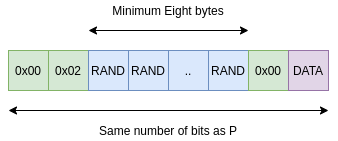
\includegraphics[width=300pt]{img/padding.png}
 \caption{PKCS padding scheme}
 \label{rPKCS}
 \end{figure}

\subsubsection{Block Handling}

ElGamal is not a common choice for encrypting larger texts, however after conversations with the lecturer, I understood that this was a requirement for this assignment. To keep the overhead to a minimum, ECB(Electronic Codebook) was chosen. An illustration of ECB can be seen in figure \ref{rECB}. If the plaintext is larger than the number of bits of P, we divide it up into blocks, encrypt them seperately, and concatenate them.
%DETTE BILDET MÅ BYTTES UT, VISER DEC OG IKKE ENC!!!!!!!!!!!!!!!!!!!!!!!!!!!!!!!!!!!!!!!!!!!
\begin{figure}[H]
 \centering
  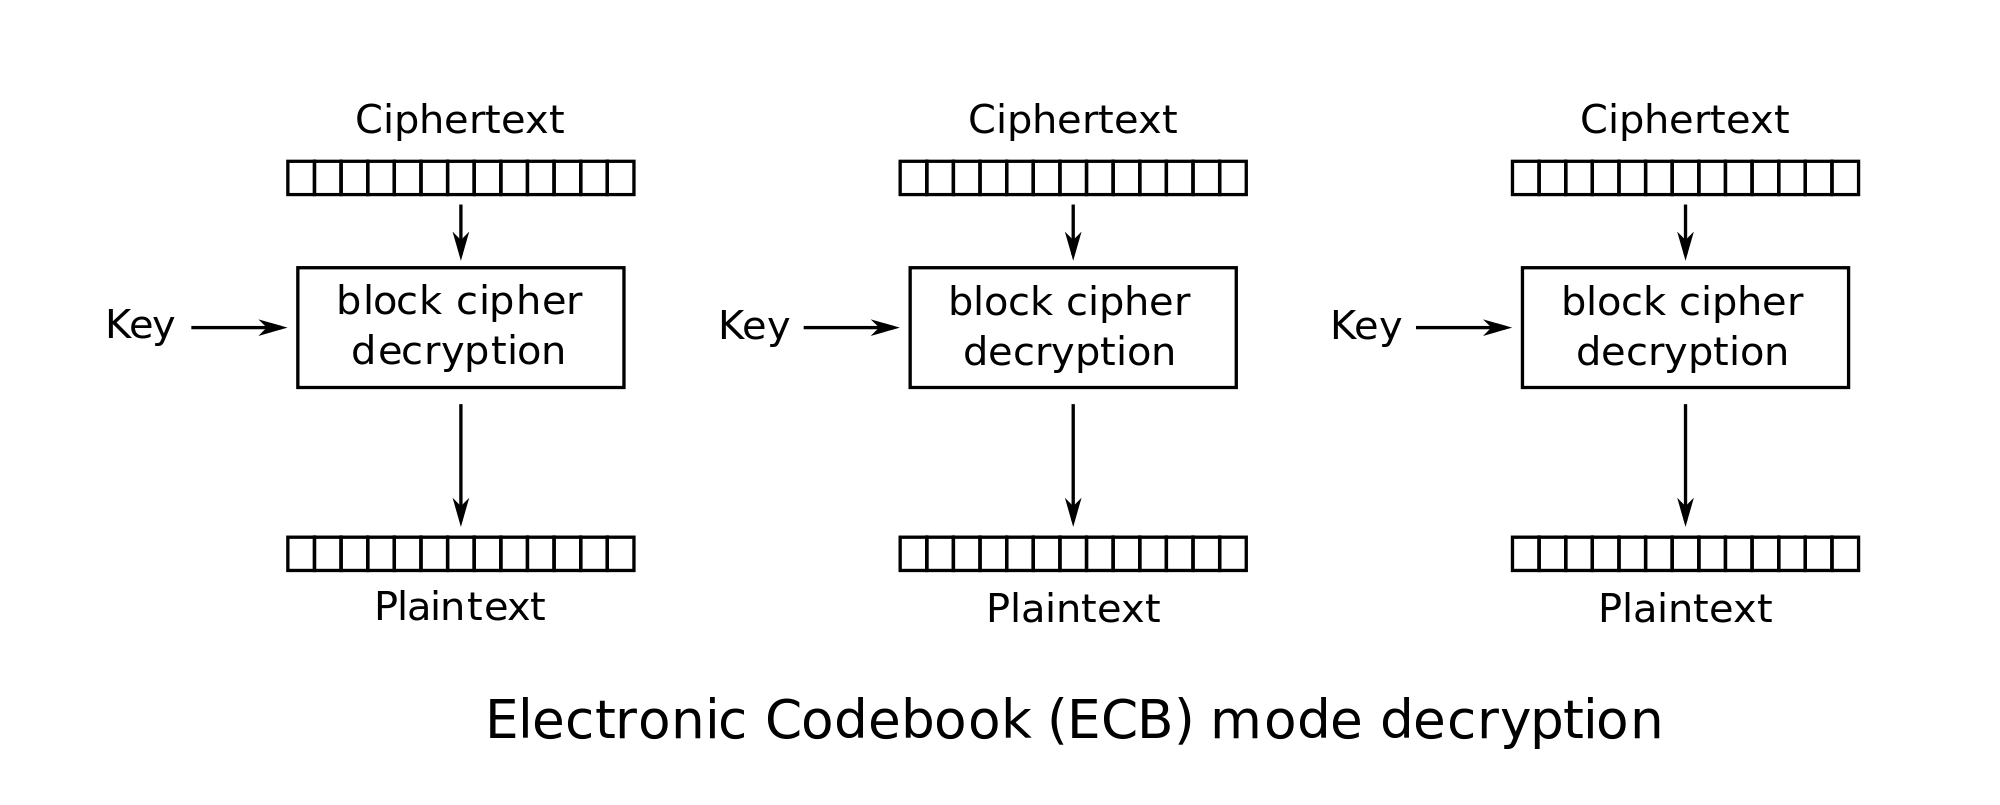
\includegraphics[width=300pt]{img/ECB.png}
 \caption{Electronic Codebook\cite{ECB}}
 \label{rECB}
 \end{figure}

An extra complication with ElGamal is that the algorithm produces two numbers, in which the size of bits may vary. In order to be able to parse the concatenated strings later, I decided to prepend zeroes to c1 and c2, until their length were at 512 bits.

Putting the padding together with Elgamal and and the post-encryption padding the full overview of this implementation encrypts a string, can be seen in figure \ref{rOVERHEAD}

\begin{figure}[H]
 \centering
  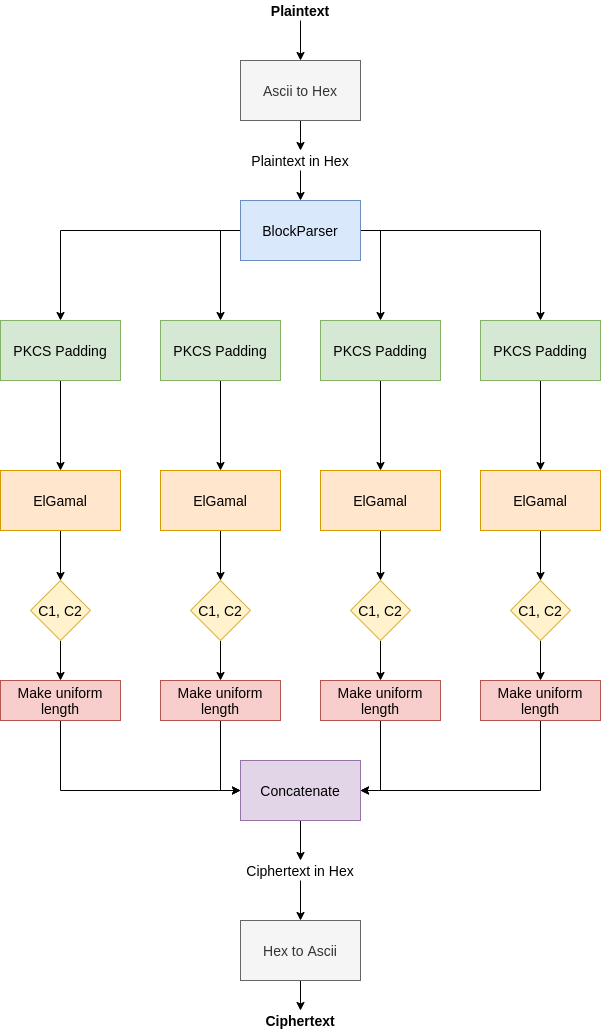
\includegraphics[width=300pt]{img/overview.png}
 \caption{Overview of the overhead}
 \label{rOVERHEAD}
 \end{figure}

\subsection{ElGamal}

Within the ElGamal implementation, most of the operations are quite trivial, and is basically the wikipedia article, translated into code.

For all of the modular exponentiation operations, I implemented the algorithm as described in psuedo code in the course book\cite{ROSEN}.

The group chosen for the implementation was
\begin{equation*}
  G =((\mathbb{Z}/P)^{*}, *)
\end{equation*}

As i could not find any resources listing good primes and generators for ElGamal, I implemented my solution with the P and g from the 512 bit encryption test vector from a github repository\cite{PG}.
\subsection{Results}

As mentioned, the implementation takes a file, encrypts it, decrypts it and writes the results to two other files. The input file and the decrypted file is also compared to make sure that they match.

Running the program looks like this:

\begin{figure}[H]
 \centering
  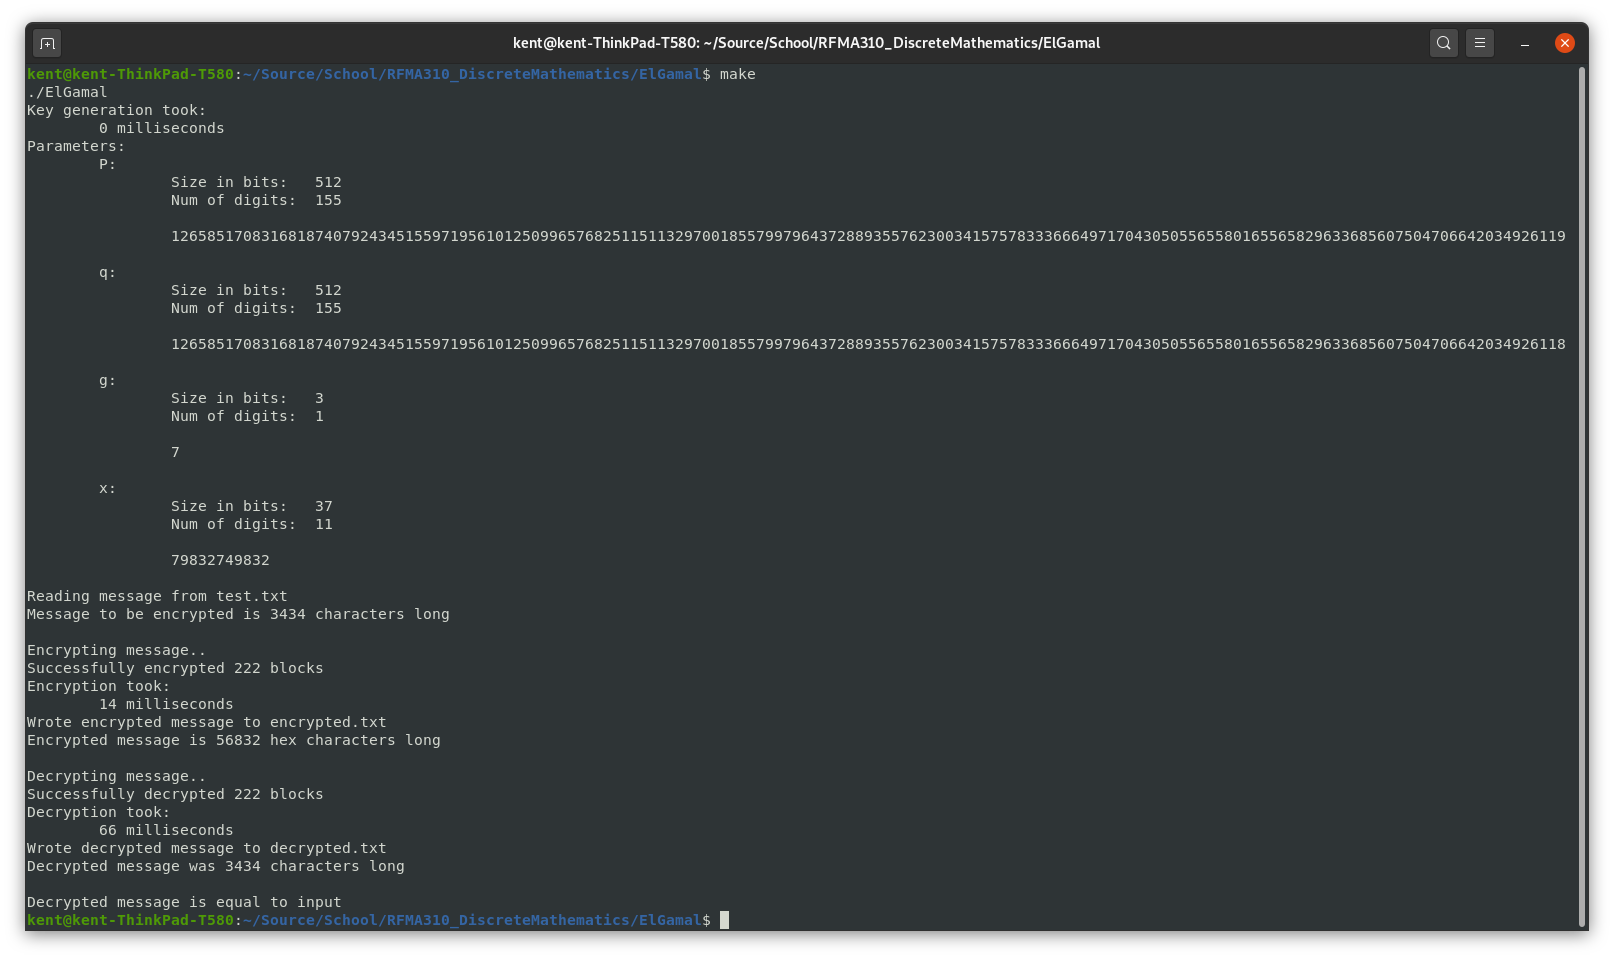
\includegraphics[width=300pt]{img/make.png}
 \caption{Running the implementation}
 \label{MAKE}
 \end{figure}
\textit{Please zoom in for closer inspection, or locate the .png added in the zip-file appended}.


The three files are too large to be included within this report, but they are located in the zip-file appended along with figures and source code.

%Konklusjon
\section{Conclusion}
In order to understand something, I would say the best way is to implement it in code. Only by truly understanding it yourself, are you able to describe to a computer how to do it. The same goes for ElGamal encryption.

I am quite satisfied with the implementation overall. It is quite efficient, as encryption usually takes around 14ms, and decryption takes around 66ms, with a 512 bit P. One should keep in mind that this is with a lot of overhead, which means that the encryption of a single block, which is more similar to a real world use of ElGamal, would be much faster.

One thing that could have been implemented was the generation of P and g. As I have implemented relatively efficient large prime generators before, generating P would not have been a problem. However, after conversations with the professor, I found that finding a good generator would be too time-consuming. A simple solution would make for a horribly inefficient program, on the other hand, a complex and useable solution would take too much time to understand, and implement.
\newpage
%Referanse
%\section{Referanser}

\nocite{*}
\bibliographystyle{plain}
\bibliography{ref}

\addcontentsline{toc}{section}{References}

\newpage

%Vedlegg
\section{Appendices}
\subsection{Sourcecode}
\begin{lstlisting}

#include <iostream>
#include <fstream>
#include <chrono>
#include "ElGamal.h"

std::string readFile(std::string fileName);
void writeFile(std::string fileName, std::string contents);

int main()
{
	//Files to be written and read
	std::string inputFile = "test.txt";
	std::string encryptFile = "encrypted.txt";
	std::string decryptFile = "decrypted.txt";

	//Seed random number generator with time.
	srand(time(0));
	try
	{
		//Set privatekey (x)
		bigInt privKey = 79832749832;

		//Generate public key (G, g, q, x)
		auto time1 = std::chrono::high_resolution_clock::now();
		auto pubKey = ElGamal::generatePublicKey(privKey);
		auto time2 = std::chrono::high_resolution_clock::now();
		std::cout << "Key generation took: \n\t" << std::chrono::duration_cast<std::chrono::milliseconds>(time2 - time1).count() << " milliseconds\n";
		ElGamal::printParameters(pubKey, privKey);

		std::cout << "Reading message from " << inputFile << "\n";
		std::string message = readFile(inputFile);
		std::cout << "Message to be encrypted is " << message.size() << " characters long\n\n";

		std::cout << "Encrypting message..\n";
		time1 = std::chrono::high_resolution_clock::now();
		auto ciphertext = ElGamal::encrypt(ElGamal::plaintextToHexString(message), pubKey);
		//STOP AND PRINT ENCRYPT TIME
		time2 = std::chrono::high_resolution_clock::now();
		std::cout << "Encryption took: \n\t" << std::chrono::duration_cast<std::chrono::milliseconds>(time2 - time1).count() << " milliseconds\n";
		writeFile(encryptFile,  ciphertext);
		std::cout << "Wrote encrypted message to " << encryptFile << "\n";
		std::cout << "Encrypted message is " << ciphertext.size() << " hex characters long\n\n";

		std::cout << "Decrypting message..\n";
		time1 = std::chrono::high_resolution_clock::now();
		auto plaintext = ElGamal::hexStringToPlaintext(ElGamal::decrypt(ciphertext, pubKey, privKey));
		time2 = std::chrono::high_resolution_clock::now();
		std::cout << "Decryption took: \n\t" << std::chrono::duration_cast<std::chrono::milliseconds>(time2 - time1).count() << " milliseconds\n";
		writeFile(decryptFile, plaintext);
		std::cout << "Wrote decrypted message to " << decryptFile << "\n";
		std::cout << "Decrypted message was " << plaintext.size() << " characters long\n\n";

		if(message == plaintext)
		{
			std::cout << "Decrypted message is equal to input\n";
		}
		else
		{
			std::cout << "Decrypted message is NOT equal to input \n";
		}
	}
	catch (std::exception& e)
  	{
    	std::cout << e.what() << '\n';
  	}
  	return 0;
}

std::string readFile(std::string fileName)
{
	std::fstream file;
	file.open(fileName);
	std::stringstream sstream;
	sstream << file.rdbuf();
	file.close();
	return sstream.str();
}

void writeFile(std::string fileName, std::string contents)
{
	std::ofstream file;
	file.open(fileName);
	file << contents;
	file.close();
}
\end{lstlisting}

\begin{lstlisting}
//ElGamal.h

#ifndef ELGAMAL_H
#define ELGAMAL_H

#include <iostream>
#include <cstdlib>
#include <ctime>
#include <math.h>
#include <gmp.h>
#include <unistd.h>
#include <algorithm>
#include <gmpxx.h>
#include <bitset>
#include <sstream>
#include <random>
#include <chrono>

//Renaming the big integer type from the Gnu Multiple Precision Library to something more readable
using bigInt = mpz_class;

namespace ElGamal
{
	struct PublicKey
	 {
		PublicKey(std::string _p, std::string _g, bigInt privKey);
	 	bigInt p;
	 	bigInt q;
	 	bigInt g;
	 	bigInt h;
	 };

	//Type for holding the two cipher strings generated by ElGamal Encryption
	struct CipherBlock
	{
		CipherBlock(bigInt c1, bigInt c2): first(c1), second(c2){}
		bigInt first;
		bigInt second;
	};

	//Main functionality
	std::string encrypt(std::string plaintext, PublicKey pubKey);
	std::string decrypt(std::string cipherText, PublicKey pubKey, bigInt privKey);

	//Padding - Implementation of the PKCS padding scheme
	bigInt PKCS(std::string message, int nBitLen);
	std::string inversePKCS(bigInt input, int nBitLen);

	//Block handling
	std::vector<bigInt> getMessageBlocks(std::string message, unsigned int pBitSize);
	CipherBlock encryptBlock(bigInt m, PublicKey pubKey);
	bigInt decryptBlock(CipherBlock c, PublicKey pubKey, bigInt privKey);
	std::string concatCipherBlocks(std::vector<CipherBlock> cipherBlocks, unsigned int pBitSize);
	std::vector<CipherBlock> parseCiphertext(std::string ciphertext, unsigned int pBitSize);

	//Helpers
	bigInt modExp(bigInt x, bigInt y, bigInt p);
	int bitCount(bigInt n);
	std::string plaintextToHexString(std::string plaintext);
	std::string hexStringToPlaintext(std::string s);

	//Generators
	bigInt generateRandomNumber(int bits);
	bigInt generateRandomNumber(bigInt min, bigInt max);
	PublicKey generatePublicKey(bigInt privKey);

	//Printers
	void printParameters(PublicKey pubKey, bigInt privKey);
	void printNumberDetails(std::string name, bigInt a);
	void printCipherBlock(CipherBlock c);
}
#endif
\end{lstlisting}

\begin{lstlisting}
//ElGamal.cpp

#include "ElGamal.h"

using namespace ElGamal;

//Constructor for public key struct, generates based on the private key
ElGamal::PublicKey::PublicKey(std::string _p, std::string _g, bigInt privKey)
{
	p = bigInt(_p, 16);
	q = p - 1;
	g = bigInt(_g, 16);
	h = modExp(g, privKey, p);
}

//Main encryption function. Takes and returns a hex-string
std::string ElGamal::encrypt(std::string plaintext, PublicKey pubKey)
{
	//Parse and pad the message, get encryptable blocks instead.
	auto blocks = getMessageBlocks(plaintext, bitCount(pubKey.p));
	std::vector<CipherBlock> cipherBlocks;

	//Encrypt each block separately
	for(auto block : blocks)
	{
		cipherBlocks.push_back(encryptBlock(block, pubKey));

	}
	//Pad (if necessary) and concatenate all cipher blocks to a single string
	auto ciphertext = concatCipherBlocks(cipherBlocks, bitCount(pubKey.p));
	std::cout << "Successfully encrypted " << blocks.size() << " blocks\n";
	return ciphertext;
}

//Separate the input string in hex into blocks relative to the size of P, and add PKCS padding scheme to the blocks
std::vector<bigInt> ElGamal::getMessageBlocks(std::string plaintext, unsigned int pBitSize)
{
	std::vector<bigInt> blocks;

	//Initial blockSize, needs to be within what is allowed by PKCS padding scheme
	unsigned int blockSize = pBitSize/8 - 11*3;

	for(int i = 0; i < plaintext.size(); i += blockSize)
	{
		//Extract substrings of suitable size
		std::string s = plaintext.substr(i, blockSize);
		//Insert a padded block into the array
		blocks.push_back(PKCS(s, pBitSize));
	}
	return blocks;
}

//PKCS\#1V1.5 padding scheme
//More detailed description at: https://www.di-mgt.com.au/rsa\_alg.html
bigInt ElGamal::PKCS(std::string message, int nBitLen)
{
	std::string binaryMessage = "";
	int keyLen = nBitLen;
	//Check that the block we are about to parse isn't to long
	if(message.size()*8 > keyLen - 11*3) throw std::invalid_argument("Message size to big in PKCS");

	//Length of the random padding, will be keylength - message size - the size of the static flags.
	int pLength = keyLen - message.size()*8 - 3*8;
	//Appending the startflags to the message
	binaryMessage += "00000000";
	binaryMessage += "00000010";
	int counter = 0;
	//Appending random bytes for as long as necessary
	while(binaryMessage.size() < (pLength + 2*8))
	{
		std::string pString = generateRandomNumber(1, pow(2, 8)-1).get_str(2);
		while (pString.size() < 8) pString.insert(0, "0");
		binaryMessage += pString;
	}

	//Appending the flag before the data
	binaryMessage += "00000000";
	//Appending the data
	for(char c : message)
	{
		binaryMessage += std::bitset<8>(c).to_string();
	}
	//Casting the binary message to a bigInt
	bigInt padded(binaryMessage, 2);
	return padded;
}

//Performs the ElGamal encryption on a single block < P
CipherBlock ElGamal::encryptBlock(bigInt m, PublicKey pubKey)
{
	if(m > pubKey.p)
	{
		throw std::invalid_argument( "m larger than p" );
	}
	//Generating random Y for each block
	bigInt y = generateRandomNumber(1, pubKey.q - 1);
	//s = h**y mod p
	bigInt s = modExp(pubKey.h, y, pubKey.p);
	//c1 = g**y mod p
	bigInt c1 = modExp(pubKey.g, y, pubKey.p);
	//c2 = m*s mod p
	bigInt c2 = modExp(m*s, 1, pubKey.p);

	return CipherBlock(c1, c2);
}

//Pad all C1 and C2 so that the length is uniform, and concatonate them into a single string
std::string ElGamal::concatCipherBlocks(std::vector<CipherBlock> cipherBlocks, unsigned int pBitSize)
{
	std::string ciphertext = "";
	unsigned int cSize = pBitSize/4;
	for(auto c : cipherBlocks)
	{
		//Casting the ciphers from bigInt to hex string
		std::string c1 = c.first.get_str(16);
		std::string c2 = c.second.get_str(16);
		//Prepending zeroes until they are of same bit size as p
		while(c1.size() < cSize) c1.insert(0, 1, '0');
		while(c2.size() < cSize) c2.insert(0, 1, '0');

		//Concatenate c1 and c2
		ciphertext += c1;
		ciphertext += c2;
	}

	return ciphertext;
}

//Main decryption function
std::string ElGamal::decrypt(std::string cipherText, PublicKey pubKey, bigInt privKey)
{
	//Parse the string into a vector of cipherblock structs
	auto cipherBlocks = parseCiphertext(cipherText, bitCount(pubKey.p));

	std::string plaintext = "";

	for(auto c : cipherBlocks)
	{
		//Decrypt each block
		bigInt m = decryptBlock(c, pubKey, privKey);
		//Remove PKCS padding
		plaintext += inversePKCS(m, bitCount(pubKey.p));
	}

	std::cout << "Successfully decrypted " << cipherBlocks.size() << " blocks\n";

	return plaintext;
}

//Separate the ciphertext into blocks of C1's and C2's
std::vector<CipherBlock> ElGamal::parseCiphertext(std::string ciphertext, unsigned int pBitSize)
{
	//Only gather substring of same amount of bits as P, and cast them to bigInts.
	//Insert into a vector of cipherblocks

	std::vector<CipherBlock> cipherBlocks;

	unsigned int cipherDigitSize = pBitSize/4;

	for(int i = 0; i < ciphertext.size(); i += cipherDigitSize*2)
	{
		auto c1 = ciphertext.substr(i, cipherDigitSize);
		auto c2 = ciphertext.substr(i+cipherDigitSize, cipherDigitSize);

		cipherBlocks.push_back(CipherBlock(bigInt(c1, 16), bigInt(c2, 16)));
	}

	return cipherBlocks;
}

//Decrypt a single block
bigInt ElGamal::decryptBlock(CipherBlock c, PublicKey pubKey, bigInt privKey)
{
	//s = c1**x mod p
	bigInt s = modExp(c.first, privKey, pubKey.p);
	//sInverse = c1**(q-x) mod p
	bigInt sInv = modExp(c.first, pubKey.q - privKey, pubKey.p);
	//m = (c2*sInverse) mod p
	bigInt m = modExp(c.second * sInv, 1, pubKey.p);

	return m;
}

//Remove the PKCS padding
std::string ElGamal::inversePKCS(bigInt input, int nBitLen)
{
	std::string data = input.get_str(2);
	//A bit of a bad solution here. As the leading zeroes will have disappeared in the casting from string to int
	//we have to prepend them back in.
	data.insert(0, "00000000000000");
	//We then remove them as they are not needed.
	//(This adding and removing is just to make it easier to understand, in real life we would just remove the bits immediately
	data.erase(0, 16);
	//Rest of data read into stringstream
	std::stringstream sstream(data);
	std::string output;
	bool paddingOver = false;

	while(sstream.good())
	{
		//Read out 8 bits at the time from the data
		std::bitset<8> bits;
		sstream >> bits;
		unsigned long i = bits.to_ulong();
		//Checking if we have reached the final all zero byte before the actual data comes
		if(i == 0 && !paddingOver)
		{
			//If that is the case, we of course set the flag that there is no more padding
			paddingOver = true;
			continue;
		}
		//Cast the byte to a char
		unsigned char c = static_cast<unsigned char>(i);
		//If the padding is over, and the character is not 0x00, we of course append it to the datastring we will return.
		if(paddingOver && c != 0x00)
		{
			output += c;
		}
	}
	return output;
}

//Modular exponentiation
//Implemented after the pseudo code in our book.
bigInt ElGamal::modExp(bigInt x, bigInt y, bigInt p)
{
	bigInt res = 1;
	bigInt power = x % p;

	std::string n = y.get_str(2);

	for(int i = n.size() - 1; i >= 0; i--)
	{
		if(n.at(i) == '1')
		{
			res = (res * power) % p;
		}
		power = (power * power) % p;
	}

	return res;
}

//Gives a public key struct based on the private key
PublicKey ElGamal::generatePublicKey(bigInt privKey)
{
	PublicKey pubKey
	(
		"F1B18AE9F7B4E08FDA9A04832F4E919D89462FD31BF12F92791A93519F75076D6CE3942689CDFF2F344CAFF0F82D01864F69F3AECF566C774CBACF728B81A227",
		"07",
		privKey
	);

	return pubKey;
}

//Needed to generate random Y
bigInt ElGamal::generateRandomNumber(bigInt min, bigInt max)
{
	return rand() % (max - min + 1) + min;
}

//Helper
std::string ElGamal::plaintextToHexString(std::string plaintext)
{
	std::stringstream stream;
	for(auto ch : plaintext)
	{
		unsigned long num = ch;
		if(num < 16) stream << 0;
		stream << std::hex << num;
	}
	std::string res(stream.str());
	return res;
}

//Helper
std::string ElGamal::hexStringToPlaintext(std::string s)
{
	std::string plain = "";
	for(int i = 0; i < s.size(); i+=2)
	{
		char temp = stoul(s.substr(i, 2), 0, 16);
		plain += temp;
	}
	return plain;
}

//Helper
int ElGamal::bitCount(bigInt n)
{
	int count = 0;
	while(n)
	{
		count++;
		n >>= 1;
	}
	return count;
}

//Printing
void ElGamal::printNumberDetails(std::string name, bigInt a)
{
	std::cout << "\t" << name << ":\n\t\tSize in bits:\t" << bitCount(a) << "\n\t\tNum of digits:\t" << a.get_str().size() << "\n\n\t\t" << a << "\n\n";
}
void ElGamal::printParameters(PublicKey pubKey, bigInt privKey)
{
	std::cout << "Parameters:\n";
	printNumberDetails("P", pubKey.p);
	printNumberDetails("q", pubKey.q);
	printNumberDetails("g", pubKey.g);
	printNumberDetails("x", privKey);
}
void ElGamal::printCipherBlock(CipherBlock c)
{
	std::cout << "CipherBlock: \n";
	printNumberDetails("C1", c.first);
	printNumberDetails("C2", c.second);
}
\end{lstlisting}
\end{document}
